%%%%%%%%%%%%%%%%%%%%%%%%%%%%%%%%%%%%%%%%%%%%%%
%Lab report writeup based on template by Derek Hildreth
%%%%%%%%%%%%%%%%%%%%%%%%%%%%%%%%%%%%%%%%%%%%%%

%\documentclass[aps,letterpape,10pt]{revtex4}
\documentclass[aps,letterpaper,10pt]{article}
%\documentclass{article}

\usepackage{graphicx} % For images
\usepackage{float}    % For tables and other floats
\usepackage{verbatim} % For comments and other
\usepackage{amsmath}  % For math
\usepackage{amssymb}  % For more math
\usepackage{fullpage} % Set margins and place page numbers at bottom center
\usepackage{subfig}   % For subfigures
\usepackage[usenames,dvipsnames]{color} % For colors and names
\usepackage{fancyhdr} %headers
\usepackage{listings} %for code
\usepackage{color} %to color code
\usepackage{wrapfig} % for inline images

%Color and code setup
\definecolor{dkgreen}{rgb}{0,0.6,0}
\definecolor{gray}{rgb}{0.5,0.5,0.5}
\definecolor{mauve}{rgb}{0.58,0,0.82}
\definecolor{codebg}{rgb}{.95,.95,.98}

\lstset{ %
	language=Python, 
	tabsize=4, 
	numbers=left,
	numberstyle=\footnotesize,
	backgroundcolor=\color{codebg},
	breaklines=true,
	breakatwhitespace=true,
	basicstyle=\small,
	numberstyle=\tiny\color{black},
	showstringspaces=false,
	keywordstyle=\color{blue}, 
	stringstyle=\color{dkgreen},
	commentstyle=\color{gray},
	frame=single,
	title = \texttt{\lstname}
	}

%%%%%%%%%%%%

%HEADER FORMATING%%%%%%%%%%%%%
\pagestyle{fancy}
\headheight 10pt
\setlength{\headsep}{20pt}
\lhead{MPHY 396 - Prof. Suzuki\\ Homework 6}
\rhead{A. Athanassiadis\\Due 2/15/2012}
%%%%%%%%%%%%%%%%%%%%%%%%

%Custom Definitions%%%%%%%%%%%%%%%
\newcommand{\ttt}{\texttt}
%%%%%%%%%%%%%%%%%%%%%%%%

\begin{document}
\section{Problem 1}
\textbf{Find the Fourier descriptor, $Z(k)$, of a circle of radius $r$.}\\

\noindent Consider that the boundary of the circle is comprised of $N$ evenly spaced points.  The circle can be parametrized in the complex plane by the equation:
\begin{eqnarray}
z(n) & = & x(n) + i\, y(n) \nonumber \\
& = & r \cos\left(\frac{2n\pi}{N}\right) + i\, r \sin\left(\frac{2n\pi}{N}\right) \nonumber \\
 & = & r e^{2\pi i\frac{n}{N}}
\end{eqnarray}

\noindent From this, the Fourier descriptor becomes
\begin{eqnarray}
Z(k) & = & \frac{1}{N} \sum_{n=0}^{N-1} r e^{2\pi i\frac{n}{N}} e^{-2\pi i\frac{n k}{N}} \nonumber \\
& = & \frac{1}{N} \sum_{n=0}^{N-1} r e^{2\pi i\frac{n}{N} (1-k)} \label{eq:FD1}\\
& = & \frac{r}{N}\left(\frac{1-e^{2\pi i(1-k)}}{1-e^{\frac{2\pi i}{N}(1-k)}}\right) \label{eq:FD2}
\end{eqnarray}

\noindent For $k=1,$ we can evaluate \eqref{eq:FD1} to get $$Z(1) = r.$$

\noindent However, if $k\neq 1$ then we need to use the expanded form in \eqref{eq:FD2}.  Noticing that the denominator is nonzero for all such $k$, and evaluating the numerator, we get $$Z(k) = 0\qquad\forall k\neq 1.$$

\noindent Therefore the complete Fourier descriptor of a centered circle with radius $r$ is
$$Z(k) =
\begin{cases}
r & k=1 \\
0& k\neq1.
\end{cases}
$$

\newpage
\section{Problem 2}
\textbf{Show the moments $M_{10}$ and $M_{01}$ are always $0$.}\\

\noindent Consider an image $I(x,y)$. Define \\
\begin{minipage}[c]{.49\textwidth}
\begin{eqnarray*}
x_0 & = & \frac{\sum_{x,y} x I(x,y)}{\sum_{x,y} I(x,y)}
\end{eqnarray*}
\end{minipage}
\begin{minipage}[c]{.49\textwidth}
\begin{eqnarray*}
y_0 & = & \frac{\sum_{x,y} y I(x,y)}{\sum_{x,y} I(x,y)}
\end{eqnarray*}
\end{minipage}
\vspace{20px}

\noindent the moments are given by\\

\begin{minipage}[c]{.49\textwidth}
\begin{eqnarray*}
M_{10} & = & \sum_{x,y} (x-x_0) I(x,y) \\ 
& = & \sum_{x,y} x I(x,y) - x_0 \sum_{x,y} I(x,y) \\
& = & \sum_{x,y} x I(x,y) - \sum_{x,y} x I(x,y) \\
& = & 0
\end{eqnarray*} 
\end{minipage}
\begin{minipage}[c]{.49\textwidth}
\begin{eqnarray*}
M_{01} & = & \sum_{x,y} (y-y_0) I(x,y) \\ 
& = & \sum_{x,y} y I(x,y) - y_0 \sum_{x,y} I(x,y) \\
& = & \sum_{x,y} y I(x,y) - \sum_{x,y} y I(x,y) \\
& = & 0
\end{eqnarray*}
\end{minipage}\\
\vspace{20px}

\noindent Thus for any image $I(x,y)$, $$M_{10}=M_{01}=0.$$

\newpage
\section{Problem 3}
\begin{minipage}[c]{.3\textwidth}
\centering
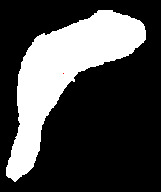
\includegraphics[width=3.5cm]{img_moment.png}
\end{minipage}
\begin{minipage}[c]{.7\textwidth}
In this problem, I calculated the first 9 principal moments of the figure to the left. They are listed below in \ttt{moments.txt}.  The code used to calculate these moments is split between \ttt{problem3.py} and \ttt{shapes.py}.  Note that $M_{02}$ is larger, as expected, because it coincides with the contribution from the spread of points in the $y$ direction.  The pixel highlighted in red is the center of mass of the image.
\lstinputlisting{moments.txt}
\end{minipage}
\lstinputlisting{problem3.py}

\section{Problem 4}
\textbf{Prove the invariance of  $\frac{Z(k)}{Z(1)}$  for $k>0$.}\\ 

\noindent Consider an $N$-element contour $z(n)$, and a linear transformation of it $z'(n) = c e^{i\theta} z(n) + z_0$ which is scaled by a factor $c$, translated by a factor $z_0$, and rotated by an angle $\theta$ about its center.  If the Fourier descriptor of $z$ is $Z(k),$ then the Fourier descriptor of $z'$ is given by 
\begin{eqnarray}
Z'(k) & = & \frac{1}{N} \sum_{n=0}^{N-1} c e^{i\theta} z(n) e^{-2\pi i \frac{n k}{N}}+ \frac{z_0}{N} \sum_{n=0}^{N-1} e^{-2\pi i \frac{n k}{N}} \nonumber \\
& = & c e^{i\theta}\sum_{n=0}^{N-1}z(n) e^{-2\pi i \frac{n k}{N}} \qquad\text{for $k>0$} \nonumber \\
& = & c e^{i\theta} Z(k)
\end{eqnarray}
Thus, for $k>0$, $$\frac{Z'(k)}{Z'(1)} = \frac{Z(k)}{Z(1)}$$ which is independent of all transformation factors.  Thus, $\frac{Z'(k)}{Z'(1)}$ is invariant to translation, rotation, and scaling.

\section{Appendix: Common Code}
The base code used for Problem 3 in this homework is contained in \ttt{shapes.py}.
\lstinputlisting{shapes.py}
\end{document} 